\documentclass[aspectratio=169]{beamer}
\usetheme{metropolis}
\usepackage{graphicx}
\usepackage{listings}
\usepackage{xcolor}
\usepackage{fontawesome5}
\usepackage{booktabs}
\usepackage{hyperref}

\definecolor{GDGoCampusblue}{HTML}{4285F4}
\definecolor{GDGoCampusgreen}{HTML}{34A853}
\definecolor{GDGoCampusyellow}{HTML}{FBBC05}
\definecolor{GDGoCampusred}{HTML}{EA4335}
\setbeamercolor{frametitle}{bg=GDGoCampusblue}
\setbeamercolor{progress bar}{fg=GDGoCampusblue,bg=gray!20}

\graphicspath{{./assets/}}

\title{Buzy AI}
\subtitle{Système d'exploitation autonome pour les organisations}
\date{GDGoCampus Gemma 4 Hackathon 2026}
\author{Destin Bir}

\begin{document}

\begin{frame}
  \titlepage
\end{frame}

\begin{frame}{Le problème}
  \begin{columns}[T]
    \column{0.6\textwidth}
    Les entreprises produisent chaque jour des \alert{contrats, factures, comptes-rendus, tableaux de bord} — dispersés entre PDF, tableurs, images et enregistrements audio.
    \vspace{1em}
    \begin{itemize}
      \item Extraire des informations exploitables prend des \alert{heures de travail manuel}
      \item Les documents sont dans \alert{des formats hétérogènes} non connectés
    \end{itemize}
    \vspace{1em}
    \textbf{Exemples de questions :}
    \begin{quote}
      ``Quel fournisseur représente le plus grand risque opérationnel le trimestre prochain ?''
    \end{quote}
    \begin{quote}
      ``Faut-il renouveler ce contrat ?''
    \end{quote}

    \column{0.4\textwidth}
    \centering
    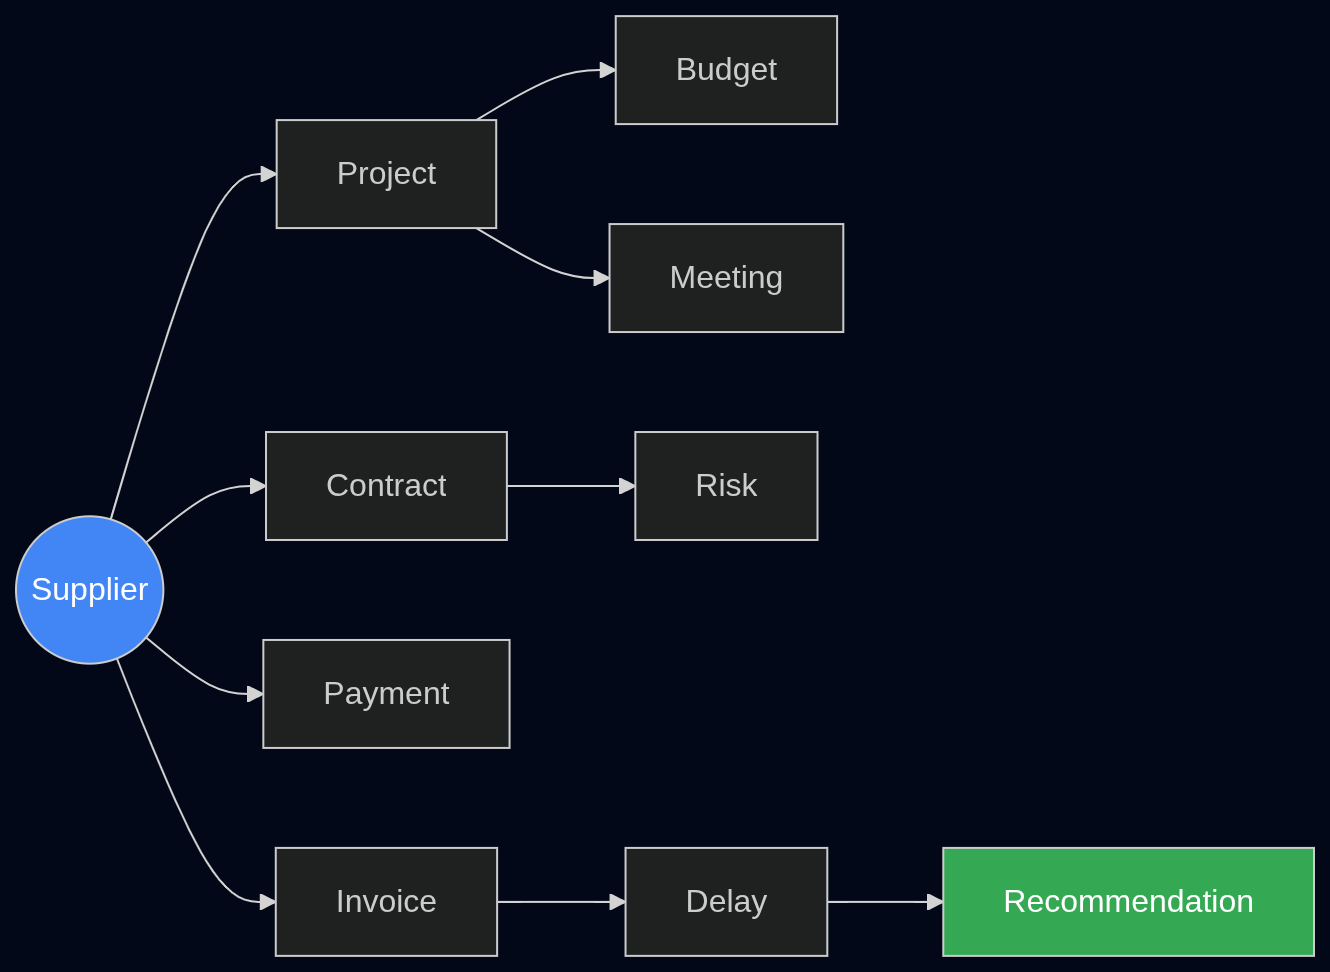
\includegraphics[width=\textwidth,height=0.7\textheight,keepaspectratio]{business_knowledge_graph.png}
  \end{columns}
\end{frame}

\begin{frame}{Solution}
  \textbf{Buzy AI} est un système de raisonnement métier multimodal qui transforme des documents bruts en décisions structurées et explicables.
  \vspace{0.5em}
  \begin{columns}[T]
    \column{0.6\textwidth}
    \begin{enumerate}
      \item \textbf{Ingestion} de documents (PDF, DOCX, TXT), images et audio
      \item \textbf{Extraction} de faits structurés via Gemma 4 Vision-Language
      \item \textbf{Construction} d'une base de connaissances légère
      \item \textbf{Recherche} des preuves pertinentes pour chaque question
      \item \textbf{Génération} de recommandations structurées avec sources
    \end{enumerate}

    \column{0.4\textwidth}
    \centering
    
\includegraphics[width=\textwidth,keepaspectratio]{architecture.png}
  \end{columns}
\end{frame}

\begin{frame}{Architecture du pipeline décisionnel}
  \centering
  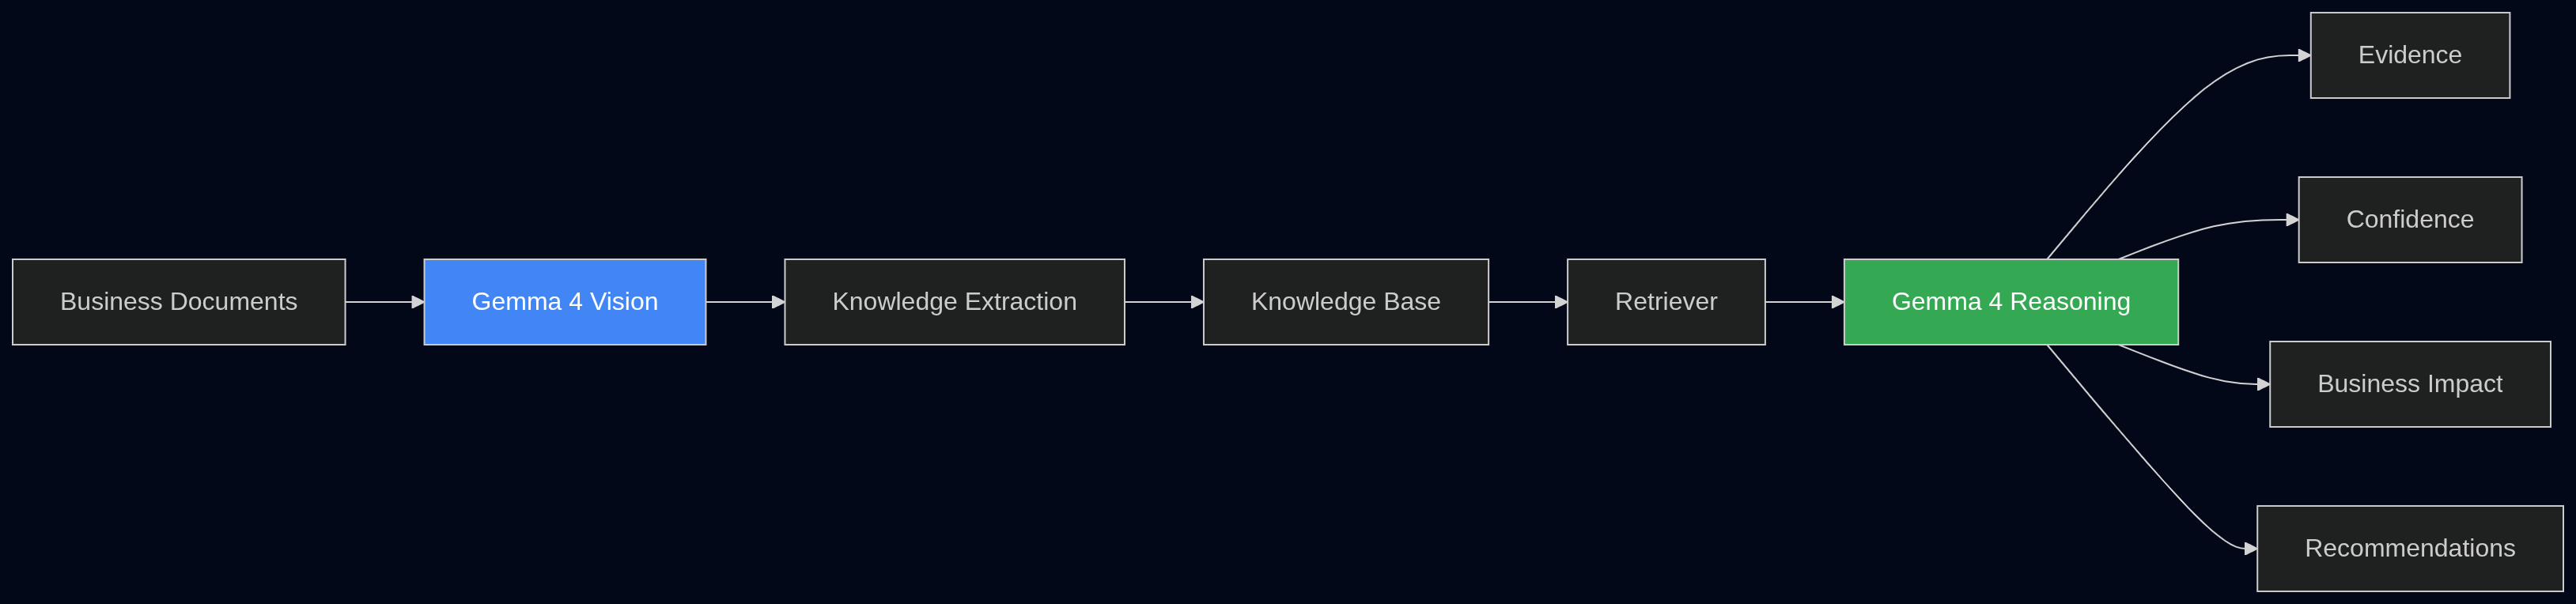
\includegraphics[width=0.75\textwidth,keepaspectratio]{business_decision_pipeline.png}
  \vspace{0.5em}
  \begin{itemize}
    \item Données brutes $\rightarrow$ analyse multimodale $\rightarrow$ extraction $\rightarrow$ base de connaissances $\rightarrow$ raisonnement $\rightarrow$ recommandations
  \end{itemize}
\end{frame}

\begin{frame}{Pipeline d'extraction de connaissances}
  \centering
  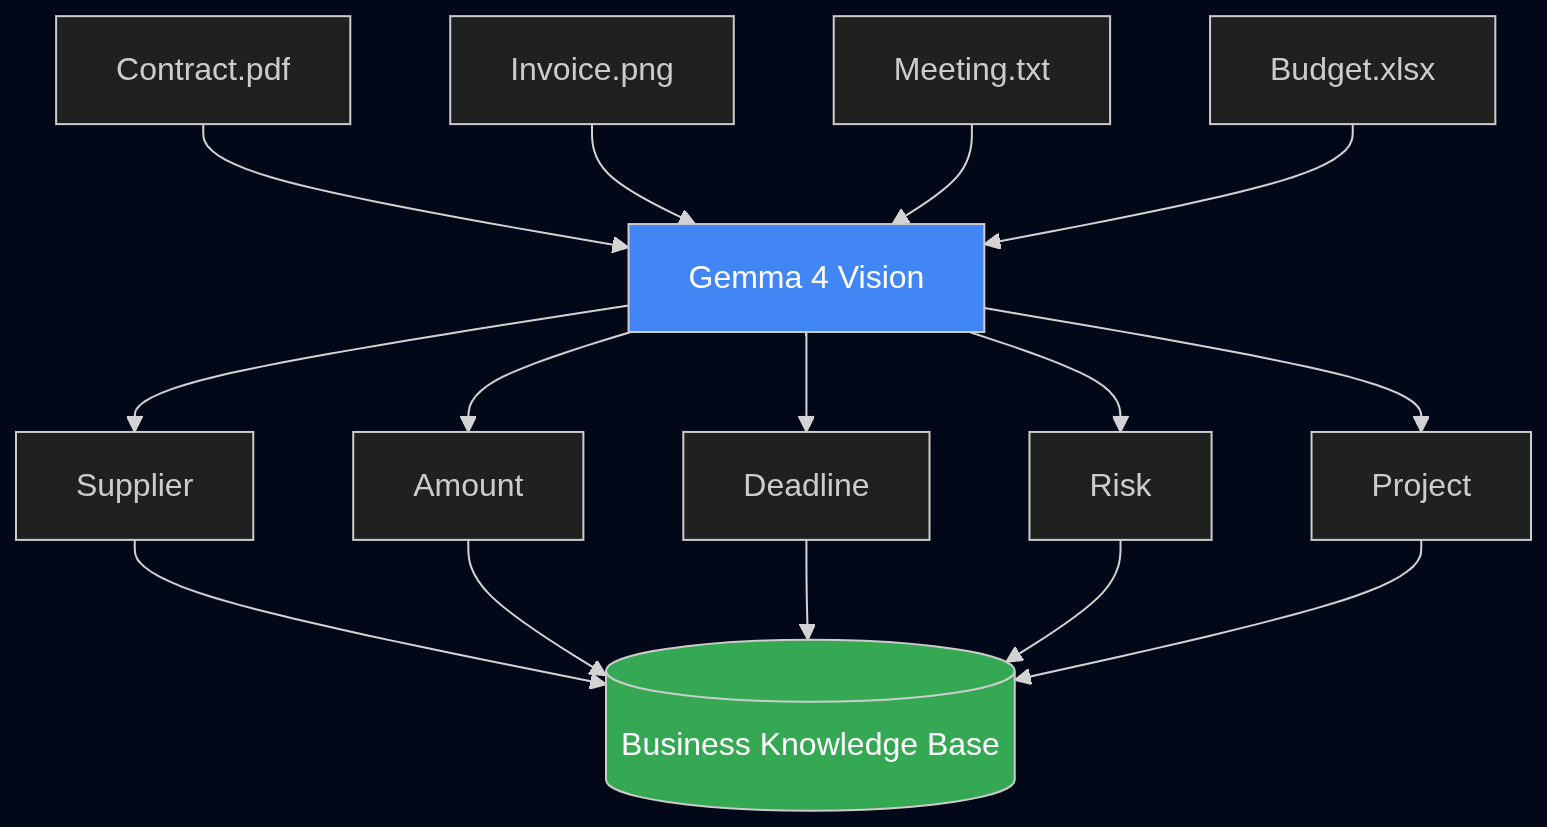
\includegraphics[width=0.65\textwidth,height=0.65\textheight,keepaspectratio]{knowledge_extraction_pipeline.png}
  \vspace{0.3em}
  \begin{itemize}
    \item Entités extraites : fournisseurs, contrats, factures, projets, risques
    \item Chaque fait est rattaché à son document source
  \end{itemize}
\end{frame}

\begin{frame}{Compréhension multimodale de documents}
  \begin{columns}[T]
    \column{0.6\textwidth}
    \textbf{Capacités Vision-Language de Gemma 4 :}
    \vspace{0.5em}
    \begin{itemize}
      \item Analyse de factures, reçus, contrats scannés
      \item Extraction JSON structurée (fournisseur, montant, dates)
      \item Traitement de tableaux de bord et captures d'écran
    \end{itemize}
    \vspace{0.5em}
    \begin{exampleblock}{Extraction de facture}
      \small
      \texttt{Entrée :} image de facture \\
      \texttt{Sortie :} \{\,"supplier": "LOGISTIQUE \& FOURNITURES SARL",\\
      \hspace*{5em}"invoice\_id": "INV-8942-FR",\\
      \hspace*{5em}"due\_date": "18 Mai 2026",\\
      \hspace*{5em}"amount": "650,00 €"\,\}
    \end{exampleblock}

    \column{0.4\textwidth}
    \centering
    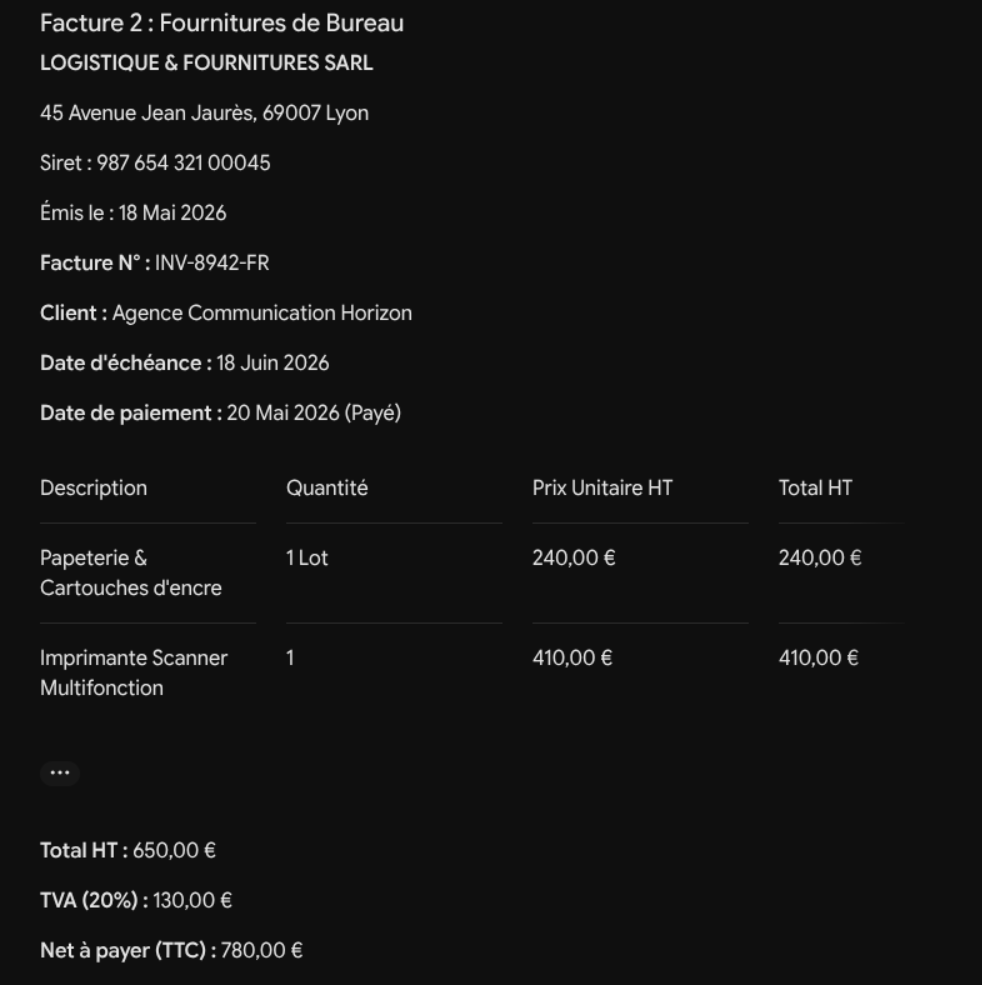
\includegraphics[width=\textwidth,keepaspectratio]{invoice_vision_extraction.png}
  \end{columns}
\end{frame}

\begin{frame}{Graphe de connaissances métier}
  \centering
  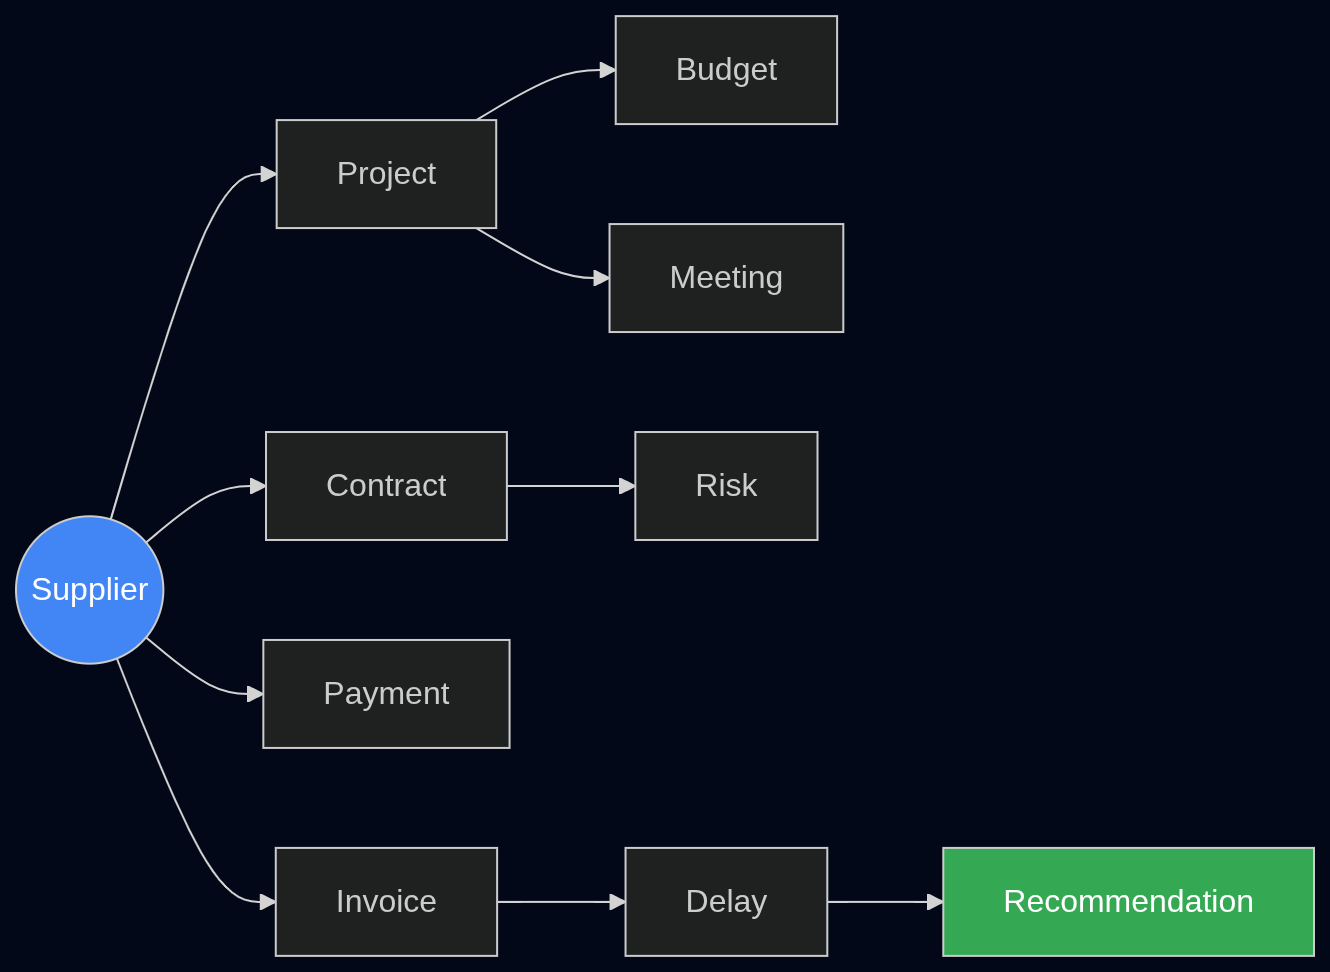
\includegraphics[width=0.8\textwidth,keepaspectratio]{business_knowledge_graph.png}
  \vspace{0.5em}
  \begin{itemize}
    \item Relations entre fournisseurs, projets, contrats et factures
    \item Types de faits : retard de paiement, expiration, risque livraison, variance budgétaire
  \end{itemize}
\end{frame}

\begin{frame}{Fine-tuning LoRA}
  \centering
  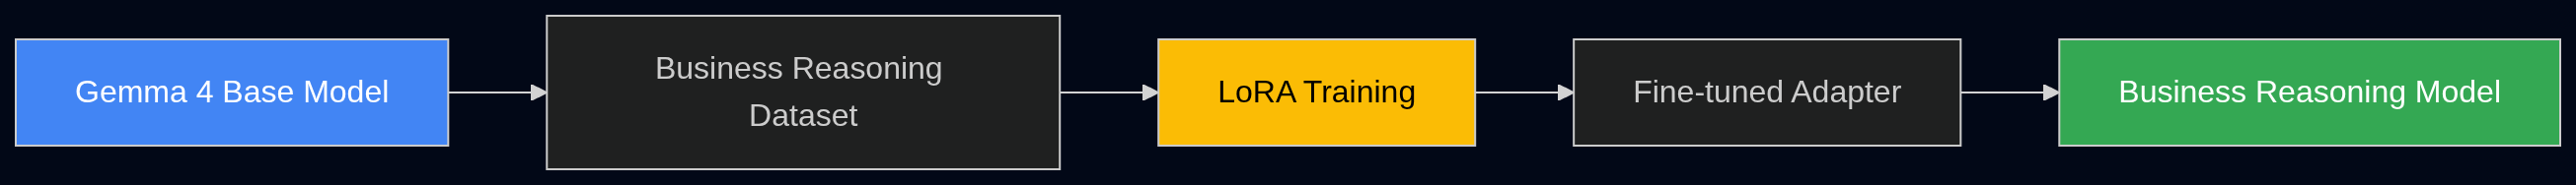
\includegraphics[width=0.5\textwidth,height=0.5\textheight,keepaspectratio]{LoRa_finetuning.png}
  \vspace{0.3em}
  \begin{columns}[T]
    \column{0.5\textwidth}
    \begin{itemize}
      \item Adaptateurs LoRA de \alert{rang 8}
      \item Couches langage seulement (vision gelée)
      \item 4 exemples de raisonnement structuré
    \end{itemize}
    \column{0.5\textwidth}
    \begin{itemize}
      \item \alert{20 époques} d'entraînement
      \item \alert{0,25\%} des paramètres (12,6M / 5,1Mds)
      \item Perte finale : \alert{0,299}
      \item Kaggle (2$\times$ T4, $\sim$57s)
    \end{itemize}
  \end{columns}
\end{frame}

\begin{frame}{Structure du jeu de données de raisonnement}
  Chaque exemple suit un schéma JSON strict :
  \vspace{0.5em}
  \begin{columns}[T]
    \column{0.5\textwidth}
    \begin{block}{Entrée}
      \small
      \texttt{Question métier :} \\
      Quel fournisseur présente \\
      le plus grand risque ? \\
      \vspace{0.3em}
      \texttt{Faits pertinents :} \\
      - 18 jours de retard de paiement \\
      - 2 projets dépendent d'Atlas \\
      - Contrat expire dans 27 jours \\
      - Instabilité de livraison signalée
    \end{block}
    \column{0.5\textwidth}
    \begin{block}{Sortie}
      \small
      \texttt{\{} \\
      \quad "evidence": [...], \\
      \quad "reasoning": [...], \\
      \quad "confidence": 0.82, \\
      \quad "business\_impact": "...", \\
      \quad "recommended\_actions": [...] \\
      \texttt{\}}
    \end{block}
  \end{columns}
\end{frame}

\begin{frame}{Raisonnement augmenté par récupération}
  \centering
  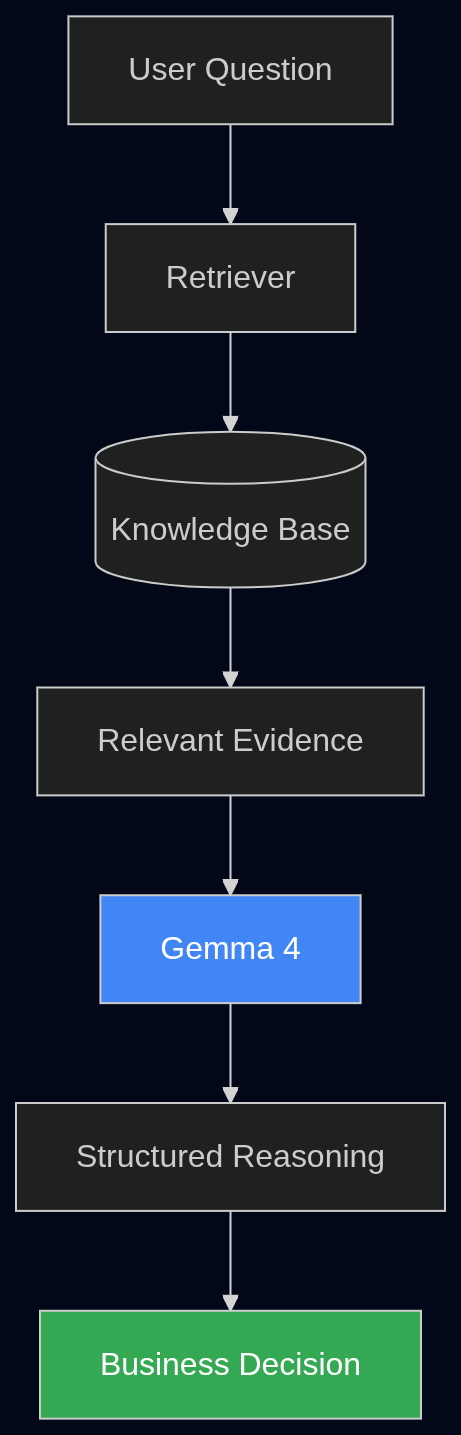
\includegraphics[width=0.65\textwidth,height=0.55\textheight,keepaspectratio]{retrieval_augmented_reasoning.png}
  \vspace{0.3em}
  \begin{itemize}
    \item Recherche par mot-clé dans la base de connaissances
    \item Gemma 4 génère une chaîne de raisonnement explicite
    \item \alert{Explicable} : preuves $\rightarrow$ raisonnement $\rightarrow$ confiance $\rightarrow$ impact $\rightarrow$ actions
  \end{itemize}
\end{frame}

\begin{frame}{Exemple d'analyse métier}
  \begin{columns}[T]
    \column{0.55\textwidth}
    \textbf{Question :} Quel fournisseur présente le plus grand risque opérationnel ?
    \vspace{0.5em}
    \begin{itemize}
      \item \alert{Preuves :} Retard de 18 jours, instabilité livraison (2 réunions), contrat expire dans 27 jours
      \item \alert{Raisonnement :} Retards répétés + dépendance exclusive du Projet Phoenix
      \item \alert{Confiance :} \textcolor{GDGoCampusgreen}{Élevée (0,82)}
    \end{itemize}

    \column{0.45\textwidth}
    \textbf{Impact :} Risque de retard de 2 semaines pour le Projet Phoenix
    \vspace{0.5em}
    \textbf{Actions :}
    \begin{enumerate}
      \item Négocier le renouvellement immédiatement
      \item Qualifier un fournisseur secondaire
      \item Renforcer le processus d'approbation des paiements
    \end{enumerate}
  \end{columns}
\end{frame}

\begin{frame}{Agent IA avec utilisation d'outils}
  \centering
  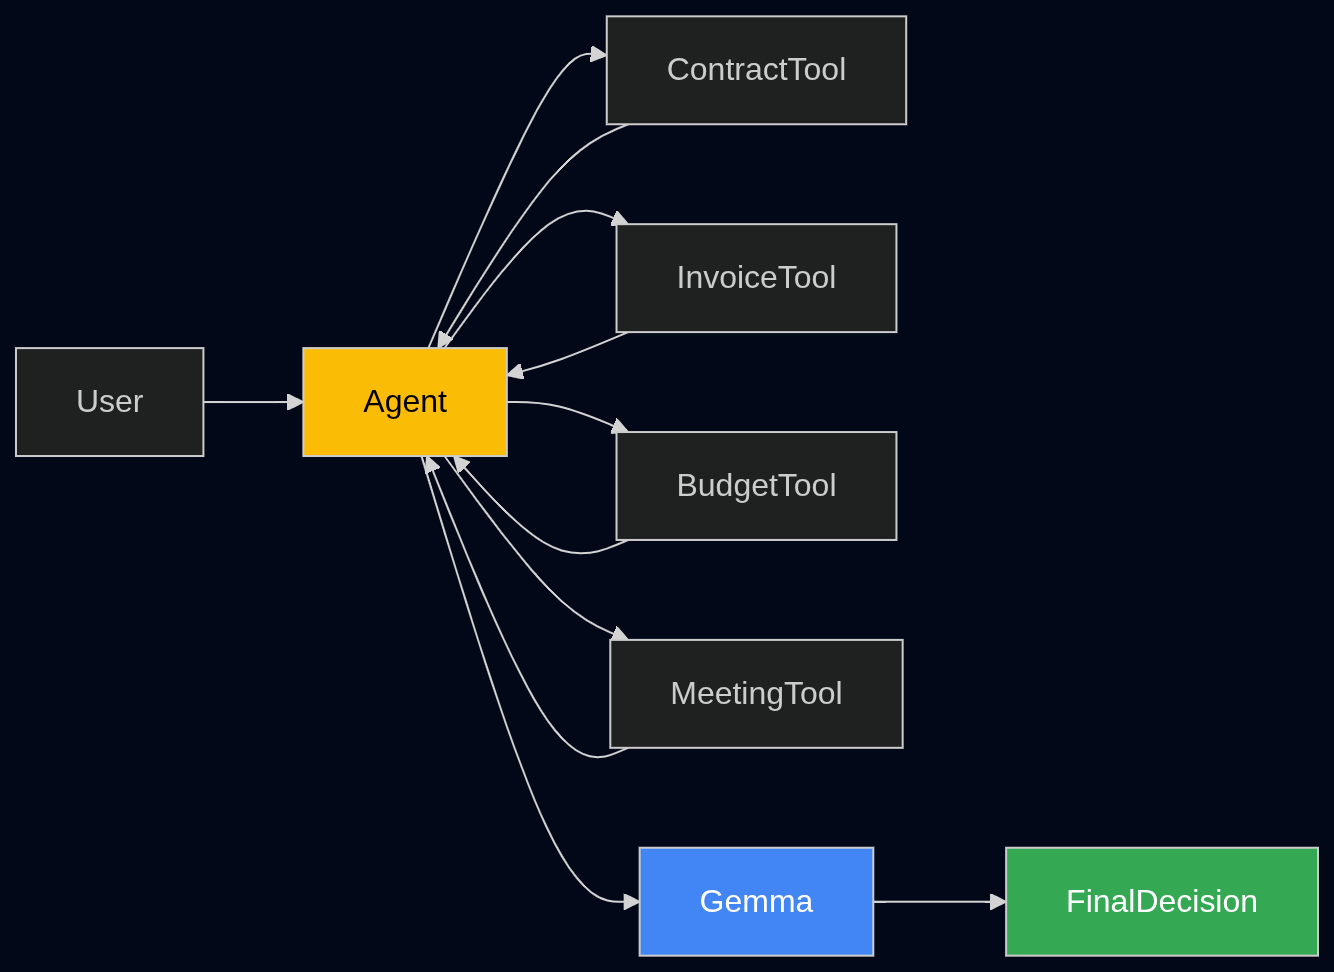
\includegraphics[width=0.6\textwidth,height=0.55\textheight,keepaspectratio]{ai_agent_workflow.png}
  \vspace{0.3em}
  \begin{itemize}
    \item Gemma 4 choisit l'outil à appeler selon la question posée
    \item Outils : \texttt{get\_invoice\_status()}, \texttt{get\_contract\_expiry()}
    \item Le résultat de l'outil est réinjecté pour générer la réponse finale
  \end{itemize}
\end{frame}

\begin{frame}{Raisonnement multilingue}
  \begin{columns}[T]
    \column{0.5\textwidth}
    \textbf{Anglais}
    \begin{quote}
      ``Which supplier represents the highest operational risk next quarter?''
    \end{quote}
    $\rightarrow$ JSON structuré avec preuves, raisonnement, confiance

    \column{0.5\textwidth}
    \textbf{Français}
    \begin{quote}
      ``Quel fournisseur représente le plus grand risque opérationnel le trimestre prochain ?''
    \end{quote}
    $\rightarrow$ Même structure JSON en français
  \end{columns}
  \vspace{1em}
  \begin{alertblock}{}
    \centering
    \alert{Même qualité de raisonnement} dans les deux langues \\
    \small (Testé avec des documents métier français)
  \end{alertblock}
\end{frame}

\begin{frame}{Application Gradio}
  \centering
  \textbf{Analyse multimodale interactive :}
  \vspace{0.5em}
  \begin{columns}[T]
    \column{0.55\textwidth}
    \begin{itemize}
      \item Import d'images, PDF/DOCX/TXT, audio
      \item Posez n'importe quelle question métier
      \item Exemples en un clic (facture, contrat, réunion)
      \item Rapport Markdown avec sources citées
    \end{itemize}
    \vspace{1em}
    \texttt{python app.py} \\
    $\rightarrow$ \texttt{http://localhost:7860}

    \column{0.45\textwidth}
    \textbf{Fonctionnalités :}
    \begin{itemize}
      \item Chargement paresseux des modèles
      \item Barre de progression Gradio
      \item Détection automatique CUDA
      \item ASR Whisper pour l'audio
      \item Galerie des images importées
    \end{itemize}
  \end{columns}
\end{frame}

\begin{frame}[fragile]{Structure du projet}
  \small
  \begin{columns}[T]
    \column{0.5\textwidth}
    \begin{lstlisting}
Buzy_Multimodal_Gemma/
  app.py
  requirements.txt
  pyproject.toml
  LICENSE
  src/
    __init__.py
    model.py
    loaders.py
    prompt.py
    inference.py
    \end{lstlisting}
    \column{0.5\textwidth}
    \begin{lstlisting}
  notebooks/
    buzy-ai-gemma4-lora.ipynb
  assets/
    architecture.png
    business_decision_pipeline.png
    knowledge_extraction_pipeline.png
    business_knowledge_graph.png
    ai_agent_workflow.png
    retrieval_augmented_reasoning.png
    LoRa_finetuning.png
    thumbnail.png
    \end{lstlisting}
  \end{columns}
\end{frame}

\begin{frame}{Stack technique}
  \centering
  \begin{tabular}{ll}
    \toprule
    \textbf{Couche} & \textbf{Technologie} \\
    \midrule
    Modèle de base & Gemma 4 (E2B-it) quantifié 4-bit \\
    Fine-tuning & LoRA via Unsloth \\
    Poids entraînés & DestinBir/buzy-ai-gemma4-lora \\
    Application & Gradio \\
    Reconnaissance vocale & Whisper (openai/whisper-small) \\
    Parsing documents & PyMuPDF, python-docx \\
    Entraînement & TRL (SFTTrainer) \\
    Plateforme & Kaggle (2$\times$ T4 GPU) \\
    \bottomrule
  \end{tabular}
\end{frame}

\begin{frame}{Résultats clés}
  \centering
  \begin{tabular}{lr}
    \toprule
    \textbf{Métrique} & \textbf{Valeur} \\
    \midrule
    Modèle de base & Gemma 4 (E2B-it)  \\
    Méthode de fine-tuning & LoRA (rang 8) \\
    Paramètres entraînés & 12,6M / 5,1Mds (0,25\%) \\
    Époques d'entraînement & 20 \\
    Perte finale & 0,299 \\
    Temps d'entraînement & $\sim$57s (2$\times$ T4) \\
    Dispositif d'inférence & CPU ou CUDA \\
    Poids du modèle & Hugging Face \\
    \bottomrule
  \end{tabular}
  \vspace{1.5em}
  \begin{alertblock}{}
    \centering
    \href{https://huggingface.co/DestinBir/buzy-ai-gemma4-lora}{Hugging Face -- DestinBir/buzy-ai-gemma4-lora}
  \end{alertblock}
\end{frame}

\begin{frame}{Liens}
  \centering
  \vspace{1em}
  \begin{tabular}{rl}
    \faicon{github} & \href{https://github.com/DestinBir/Buzy_Multimodal_Gemma}{github.com/DestinBir/Buzy\_Multimodal\_Gemma} \\[1em]
    \faicon{huggingface} & \href{https://huggingface.co/DestinBir/buzy-ai-gemma4-lora}{huggingface.co/DestinBir/buzy-ai-gemma4-lora} \\[1em]
    \faicon{kaggle} & \href{https://www.kaggle.com/code/destinbir1/buzy-ai-gemma4-lora}{kaggle.com/destinbir1/buzy-ai-gemma4-lora}
  \end{tabular}
  \vspace{2em}
  \begin{center}
    \Large Merci ! \\[0.5em]
    \normalsize GDGoCampus Gemma 4 Hackathon 2026 \\[0.5em]
    \small Propulsé par \href{https://ai.google.dev/gemma}{Gemma 4} de Google
  \end{center}
\end{frame}

\end{document}
